\documentclass{article}

\usepackage{amsmath}
\usepackage{amssymb}
\usepackage{float}
\usepackage{graphicx}
\usepackage{tikz}
\usepackage{textpos}

\usepackage[colorlinks=true, allcolors=blue]{hyperref}

\title{Lista 2}
\author{Luís Felipe Ramos Ferreira}
\date{\href{mailto:lframos.lf@gmail.com}{\texttt{lframos.lf@gmail.com}}
}

\begin{document}

\maketitle

\begin{itemize}
	\item (4.5.1)
	      \begin{itemize}
		      \item \(R(3)\)

		            Inicialmente, note que a seguinte 2-coloração do \(K_5\) não possui uma clique de tamanho 3 monocromática, portanto
		            \(R(3) > 5\).

		            \begin{figure}[H]
			            \centering
			            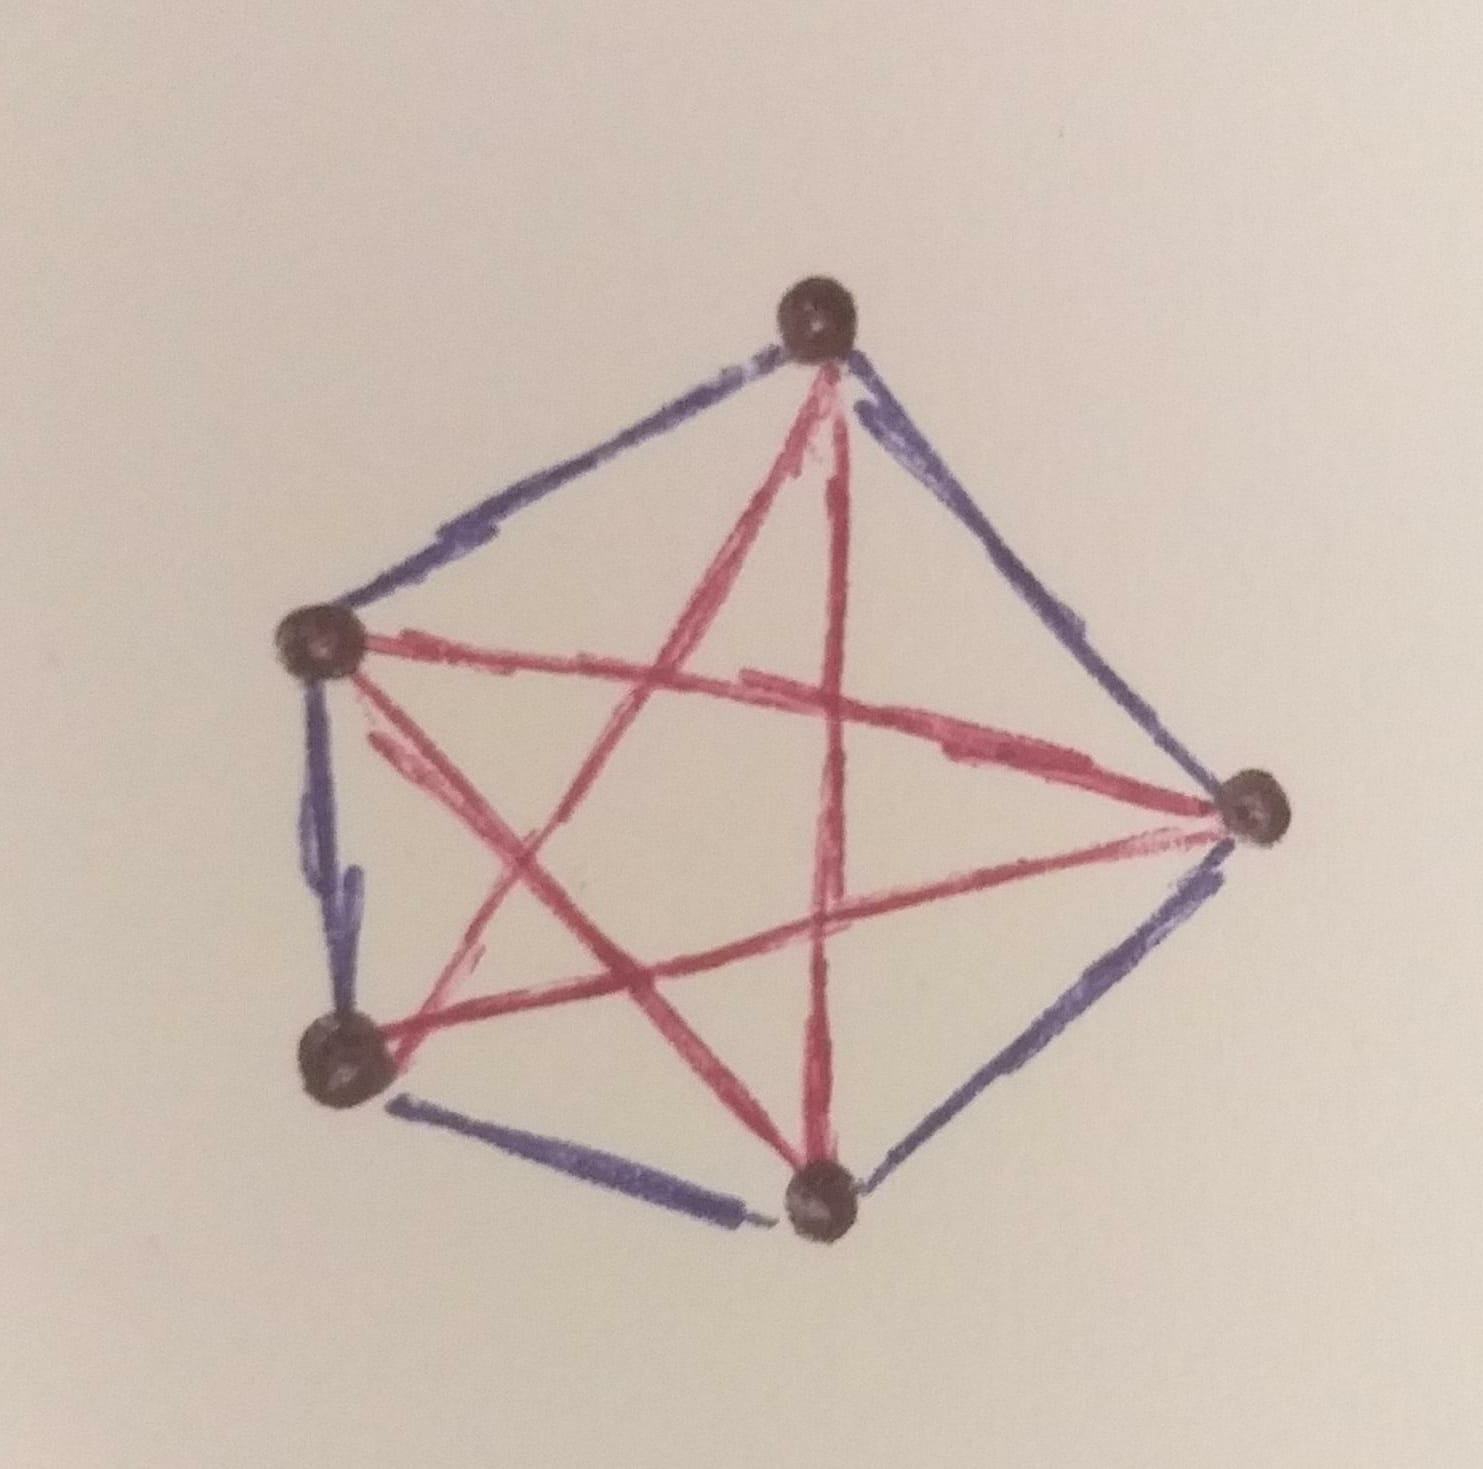
\includegraphics[width=0.8\textwidth]{images/1a.jpeg}
			            \caption{\(K_5\) 2-colorido}
		            \end{figure}

		            No entanto, sabemos pelo fato 4.0.1 do livro que o toda 2-coloração do \(K_6\) possui um triângulo monocromático, logo \(R(3) = 6\).
		            A prova funciona da seguinte forma: seja \(v\) um vértice de \(K_6\). Pelo princípio da casa dos pombos, das 5 arestas incidentes a \(v\),
		            ao menos 3 possuem a mesma cor. Vamos dizer que é a cor 1. Sejam \(x, y, z\) vizinhos de \(v\) com a aresta com cor 1. Se qualquer uma das arestas
		            \(xy, xz, yz\) for da cor 1, temos um triângulo de cor 1. Caso contrário, o triângulo formado pelos vértices \(x, y, z\) é monocromático na outra cor,
		            chamemos ela de 2. Logo, toda 2-coloração do \(K_6\) possui um triângulo monocromático.

		      \item \(R(3, 4)\)

		            Inicialmente, vamos notar que \(R(3, 4)\) é maior que 8, e isso pode ser notado pela 2-coloração do \(K_8\) abaixo em que
		            não existe uma clique de tamanho 3 vermelha e nem uma clique de tamanho 4 azul (Na imagem, o primeiro grafo tem apenas as arestas vermelhas
		            e o segundo seri ao complemento do primeiro grafo, em que as arestas são azuis).

		            \begin{figure}[H]
			            \centering
			            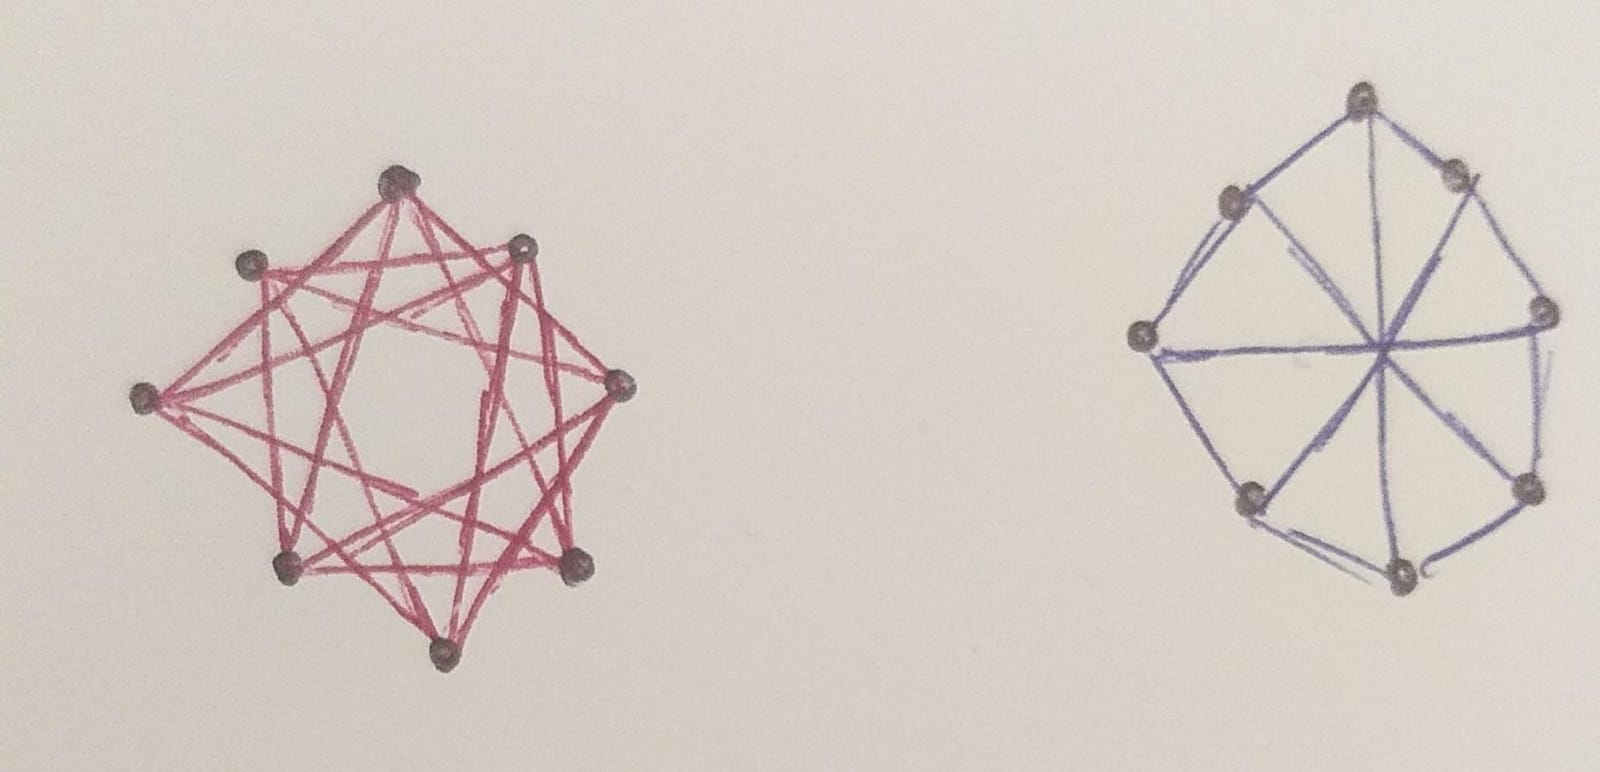
\includegraphics[width=0.8\textwidth]{images/1b.jpeg}
			            \caption{\(K_8\) 2-colorido}
		            \end{figure}

		            Vamos provar agora que \(R(3, 4) \leq 10\), em particular, mostrar que para um grafo completo de 10 vértices sempre teremos um triângulo
		            vermelho ou uma clique de tamanho 4 azul. Depois, com uma pequena variação, mostraremos que \(R(3,4) \leq 9\), o que conclui a prova.

		            Seja \(A\) um vértice qualquer de um \(K_{10}\) 2-colorido com vermelho e azul. \(A\) possui nove vizinhos e das arestas que o conectam a seus vizinhos,
		            sabemos que ao menos 6 são azuis ou ao menos 4 são vermelhas (isso porque no total precisamos ter 9 arestas, uma para cada vizinho). Suponhamos o caso em que
		            \(A\) possui 4 arestas vermelhas o conectando a seus vizinhos. Se existir uma aresta vermelha entre esses vizinhos, então existe um triângulo vermelho no grafo. Caso
		            contrário, todas as arestas entre os 4 vértices são azuis, logo existe uma clique de tamanho 4 de cor azul. Seja agora o caso em que \(A\) possui
		            6 arestas de cor azul o conectando a seus vizinhos. Sabemos que \(R(3, 3) = 6\), logo, entre esses vizinhos, há um triângulo vermelhor ou azul. Se for vermelho,
		            já perdemos, se for azul, note que ele forma uma clique de tamanho 4 azul junto com \(A\). Logo, \(10\) é um limite superior para \(R(3, 4)\).

		            Consideremos agora o caso do \(K_9\). Note que os argumentos usados anteriormente servem da mesma maneira, exceto pelo caso em que, para todo vértice \(A\),
		            exista exatamente 5 arestas azuis e 3 vermelhas saindo dele. Nesse caso, para cada vértice teremos três arestas vermelhas, e como são 9 vértices, temos \(3 * 9 = 27\). Como cada arestas
		            é contada duas vezes, precisamos dividir por dois, obtendo assim um número \(\frac{27}{2}\)(não inteiro) de arestas, o que é um absurdo. Logo, \(R(3, 4) \leq 9\)

		      \item \(R(4, 4)\)

		            Sabemos pelo lema 4.1.3 do livro que, para todo \(s, t \geq 2\), temos:
		            \[R(s, t) \leq R(s - 1, t) + R(s, t - 1)\]

		            Logo, temos que \(R(4, 4) \leq R(3, 4) + R(4, 3) = 2*R(3, 4) = 2*9 = 18\). Mostramos no exercício anterior
		            que \(R(3, 4) = 9\).
		            No entanto, vamos mostrar que existe uma 2-coloração de \(K_{17}\) tal que não existe uma clique de tamanho 4 nem vermelha nem azul, mostrando assim
		            que \(R(4, 4) = 18\). A imagem abaixo,
		            retirada \href{https://www.cut-the-knot.org/arithmetic/combinatorics/Ramsey44.shtml}{deste site}, apresenta tal grafo e sua coloração.

		            \begin{figure}[H]
			            \centering
			            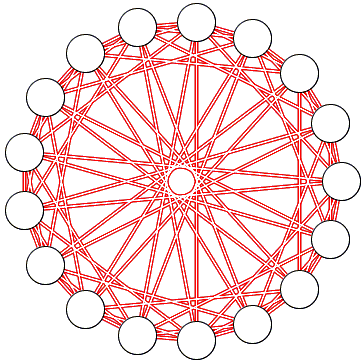
\includegraphics[width=0.4\textwidth]{images/r441.jpeg}
			            \caption{\(K_{17}\) arestas vermelhas}
		            \end{figure}

		            \begin{figure}[H]
			            \centering
			            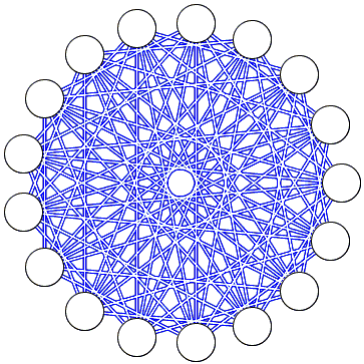
\includegraphics[width=0.4\textwidth]{images/r442.jpeg}
			            \caption{\(K_{17}\) arestas azuis}
		            \end{figure}

	      \end{itemize}

	\item (4.5.2)

	      \begin{itemize}
		      \item \(R(K_3, C_4)\)

		            Inicialmente, note que \(R(K_3, C_4) > 6\), uma vez que a 2-coloração do \(K_6\) abaixo não contêm \(K_3\) vermelho nem
		            \(C_4\) azul. Isso pois as arestas azuis formam um \(2 K_3\) e as arestas vermelhas foram um bipartido \(K_{3, 3}\).


		            \begin{figure}[H]
			            \centering
			            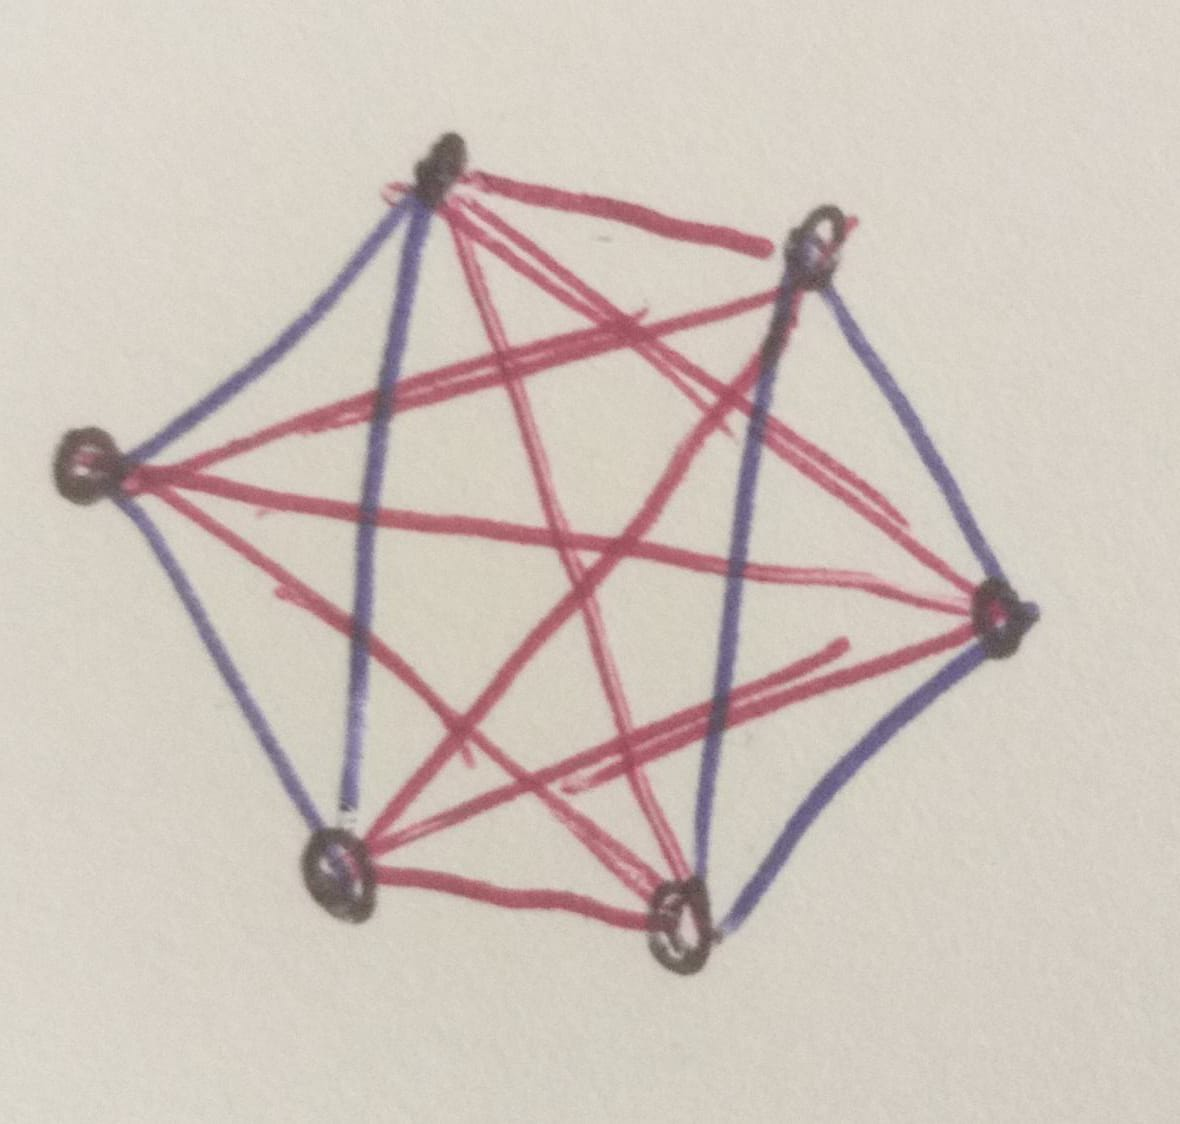
\includegraphics[width=0.5\textwidth]{images/k6.jpeg}
			            \caption{\(K_6\) 2-colorido}
		            \end{figure}

		            Seja agora um \(K_7\) 2-colorido. Como \(R(3) = 6\), sabemos que deve existir nessa 2-coloração ou um \(K_3\) vermelho ou um azul. Se for vermlho acabamos,
		            então vamos assumir que é azul. Sejam \(W = \{w_1, w_2, w_3\}\) os vértices desse \(K_3\) azul e \( V = \{v_1, v_2, v_3, v_4\}\) os vértices que sobraram no \(K_7\). Se \(V\) formar
		            uma clique azul, temos um \(C_4\) azul e acabamos. Logo vamos assumir que existe uma arestas vermelha entre vértices de \(V\). Sem perda de generalidade, vamos assumir
		            que é entre \(v_1\) e \(v_2\). Note também que para qualquer \(v \in V\), se ele possuir duas ou mais arestas azuis indo para \(W\), teríamos um \(C_4\)
		            azul formado por \(\{v, w_1, w_2, w_3\}\), então assumimos que existe no máximo uma aresta azul dessa forma, o que implica em ao menos duas arestas vermelhas
		            dessa forma. Note, no entanto, que \(v_1\) e \(v_2\) compartilham um vizinho \(w \in W\) de tal modo que \(v_1w\) e \(v_2w\) são vermelhas,
		            pelo princípio a casa dos pombos. Como \(v_1v_2\) é vermlha, temos um \(K_3\) vermelho. Logo, \(R(K_3, C_4) = 7\), como queríamos demonstrar.

		      \item \(R(K_3, C_5)\)

		            Primeiramente, vamos mostrar que \(R(K_3, C_5) > 8\) ao mostrar uma 2-coloração de um \(K_8\) tal que não existe um
		            \(K_3\) vermelho e nem um \(C_5\) azul. Tal grafo esta na imagem abaixo. Note que as arestas azuis formam 2 \(K_4\), logo é impossível
		            ter um \(C_5\) azul. Como as arestas vermelhas formam um grafo bipartido, não há como existir um \(K_3 = C_3\) vermelho.

		            \begin{figure}[H]
			            \centering
			            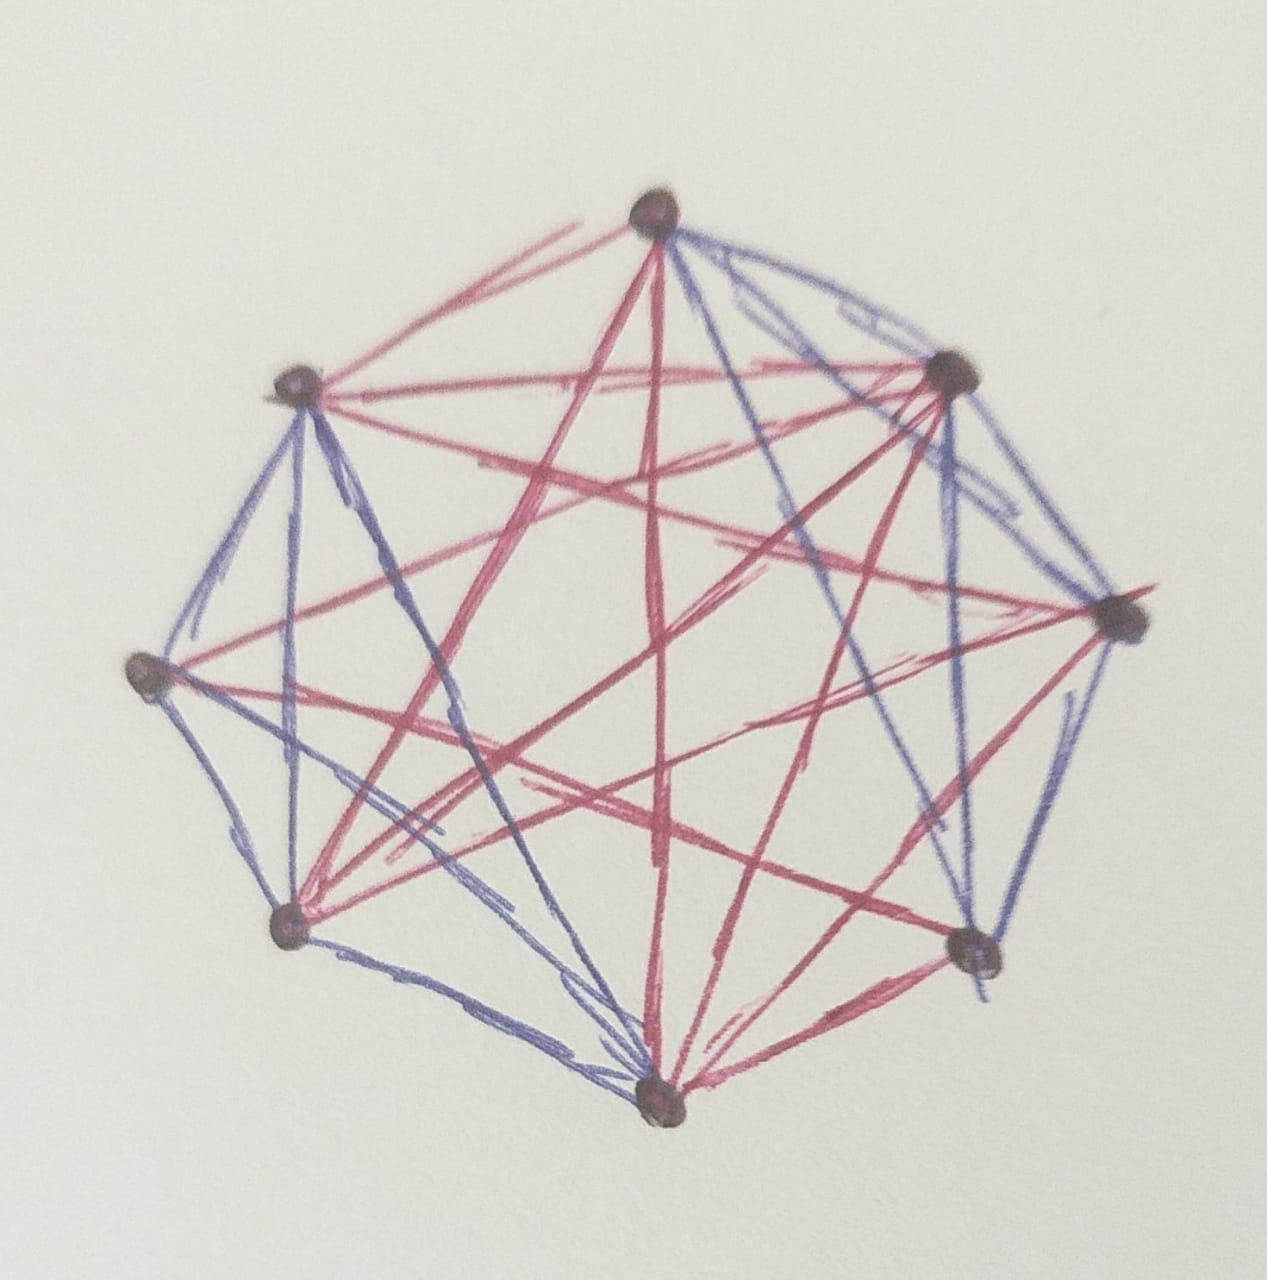
\includegraphics[width=0.5\textwidth]{images/k8.jpeg}
			            \caption{\(K_8\) 2-colorido}
		            \end{figure}

		            Seja agora um \(K_9\) com uma 2-coloração. Vamos lembrar que \(R(3, 4) = 9\), como demonstramos no exercício anterior. Logo, como se trata
		            de um \(K_9\), se não existisse um \(K_4\) azul teríamos um \(K_3\) vermelho e acabamos. Logo, vamos assumir agora que existe um \(K_4\) azul na coloração.
		            Sejam \(w_i\) para todo \(i \in \{1, 2, 3, 4\}\) os vértices nesse \(K_4\) e \(v_j\) para todo \(j \in \{1, 2, 3, 4, 5\}\) os outros vértices
		            do grafo. Se todas as arestas entre qualquer dois vértices \(v_a\) e \(v_b\) for azul, temos um \(C_5\) azul e acabamos, logo vamos assumir que existe ao menos uma aresta vermelha
		            entre um \(v_a\) e um \(v_b\). Vamos assumir sem perda de generalidade que se tratam de \(v_1\) e \(v_2\).

		            Note também que se existirem duas arestas azuis saindo de algum \(v_j\) indo para o conjunto \(\{w_1, w_2, w_3, w_4\}\), então existe um \(C_5\) azul,
		            logo podemos assumir a partir de agora que existem no máximo uma aresta azul nesse sentido, o que implica em existirem ao menos 3 arestas vermelhas nesse sentido. No entanto,
		            isso quer dizer que \(v_1\) e \(v_2\) possuem um vizinho em comum \(w_i\) de modo que \(v_1w_i\) e \(v_2w_i\) são vermelhas. Como \(v_1v_2\) também é vermelha,
		            achamos um triângulo vermelho. Logo, \(R(K_3, C_5) \leq 9\), o que implica, com o que sabemos de antes, em \(R(K_3, C_5) = 9\), como queríamos demonstrar.

	      \end{itemize}
	\item (4.5.3)

	      Sabemos que \(R(3) = 6\), logo, sabemos que o \(K_5\) não contêm \(K_3\) monocromático, logo \(\binom{5}{2} = 10\) é um limite inferior para o maior número de arestas que um grafo
	      pode ter e não possui \(K_3\) monocromático. Também, sabemos que, como \(R(3) = 6\), se \(G\) possui uma clique de tamanho 6, com certeza existirá um \(K_3\) monocromático em uma 2-coloração
	      de suas arestas, logo um \(K_6\) não pode aparecer em sua estrutura.

	      Poranto, queremos saber o maior número de arestas que um grafo com \(n\) vértices pode ter para que ele não possua \(K_6\) como subgrafo, e esse é exatamente o extremal de \(n\) e \(K_6\), isto é, \(ex(n, K_6)\), que é o número de arestas do grafo
	      \(k\)-partido de \(n\) vértices.
	      Pelo Teorema de Turán, sabemos que, se \(k\) divide \(n\):

	      \[ex(n, K_{k+1}) = (1 - \frac{1}{k})\frac{n^2}{2}\]
	      \[ex(n, K_{5+1}) = (1 - \frac{1}{5})\frac{n^2}{2} = \frac{4}{5}\frac{n^2}{2} = \frac{2n^2}{5}\]

	      Se \(k\) não divide \(n\), toda partição do grafo \(k\)-partido tem tamanho \(\lfloor \frac{n}{k} \rfloor\) ou \(\lceil \frac{n}{k} \rceil\), que possui um valor aproximadamente igual ao anterior, de \((1 - \frac{1}{k})\frac{n^2}{2}\).


	\item (4.5.4)

	      Queremos mostrar que \(R_r(3) \geq 5^{\frac{r}{2}}\). Sabemos pelo teorema 4.1.6 do livro que \(R_r{3} \geq 2^r\).
	\item (4.5.5)

	      Sabemos que \(R(t)\) é o menor \(n\) tal que toda 2-coloração de \(K_n\) contêm uma cópia monocromática de \(K_t\). Logo, se pegarmos o \(K_n\) em que \(n = R(t)\), seu número de arestas é \(\binom{n}{2}\). Obviamente temos que
	      \(\hat{r} \leq \binom{n}{2}\), pois \(K_n\) é um grafo tal que \(K_n \rightarrow K_t\). CONTINUAR

	\item (4.5.6)
	\item (4.5.7)

	      Inicialmente, vamos notar que existe um \(N \in \mathbb{N}\) tal que a partir desse \(N\) o teorema vale para \(r\), e esse \(N\) é chamado de número de
	      Schur. Sabemos pelo teorema de Ramsey que \(n = R_r(3)\) é um inteiro, que existe, tal que
	      toda r-coloração de \(K_n\) contêm uma cópia monocromático de \(K_3\).
	      Considere então o conjunto \(\{1, \dots, n\}\) e uma r-coloração dele.

	      Vamos colorir o \(K_n\) da seguinte maneira. Para cada aresta \(v_iv_j \in V(K_n)\), colorimos ela com a cor \(c\) se \(|i - j|\) foi colorido com a cor
	      \(c\) na r-coloração anterior dos inteiros de 1 até \(n\). Pelo teorema de Ramsey, sabemos que essa coloração de \(K_n\) contêm um triângulo monocromático.
	      Sejam \(v_a, v_b, v_c\), com \(a > b > c\) os vértices queformam esse triângulo, e suponha que ele foi colorido com a cor \(c\). Logo,
	      \(a - b, b - c, a - c\) são valores coloridos com a mesma cor no particionamento dos inteiros de 1 até \(n\). Note, no entanto, que
	      \(a - b + b - c = a - c\), ou seja, se tomarmos \(x = a - b\), \(y = b - c\) e \(z = a - c\), encontramos a tripla \(\{x,y,z\}\), o que prova o
	      teorema de Schur, como queríamos demonstrar.

	\item (4.5.8) OPCIONAL
	\item (4.5.9)
	\item (4.5.10)

	      Não, essa afirmativa é falsa.
\end{itemize}

\end{document}
